\documentclass{article}
\usepackage[utf8]{inputenc}

\usepackage[utf8]{inputenc}
\usepackage[margin=1in]{geometry}
\usepackage{amsmath}
\usepackage{amssymb}
\usepackage{minitoc}
\usepackage{booktabs}
\usepackage[labelfont=bf, skip=5pt, font=small]{caption}
\usepackage{subcaption}
\usepackage{graphicx}
\usepackage{fancyhdr}
\usepackage{tabu}
\usepackage{dirtytalk}
\usepackage{hyperref}

\setlength{\parskip}{0.5em}
\setlength{\parindent}{0em}
\usepackage[utf8]{inputenc}
\usepackage[T1]{fontenc}
\usepackage[french]{babel}
\usepackage{fullpage}
\usepackage{color}
\usepackage[table]{xcolor}
\usepackage{listings}
\usepackage{graphicx}
 \usepackage{float}
\definecolor{darkWhite}{rgb}{0.94,0.94,0.94}
 
\lstset{
  aboveskip=3mm,
  belowskip=-2mm,
  backgroundcolor=\color{darkWhite},
  basicstyle=\footnotesize,
  breakatwhitespace=false,
  breaklines=true,
  captionpos=b,
  commentstyle=\color{red},
  deletekeywords={...},
  escapeinside={\%*}{*)},
  extendedchars=true,
  framexleftmargin=16pt,
  framextopmargin=3pt,
  framexbottommargin=6pt,
  frame=tb,
  keepspaces=true,
  keywordstyle=\color{blue},
  language=C,
  literate=
  {²}{{\textsuperscript{2}}}1
  {⁴}{{\textsuperscript{4}}}1
  {⁶}{{\textsuperscript{6}}}1
  {⁸}{{\textsuperscript{8}}}1
  {€}{{\euro{}}}1
  {é}{{\'e}}1
  {è}{{\`{e}}}1
  {ê}{{\^{e}}}1
  {ë}{{\¨{e}}}1
  {É}{{\'{E}}}1
  {Ê}{{\^{E}}}1
  {û}{{\^{u}}}1
  {ù}{{\`{u}}}1
  {â}{{\^{a}}}1
  {à}{{\`{a}}}1
  {á}{{\'{a}}}1
  {ã}{{\~{a}}}1
  {Á}{{\'{A}}}1
  {Â}{{\^{A}}}1
  {Ã}{{\~{A}}}1
  {ç}{{\c{c}}}1
  {Ç}{{\c{C}}}1
  {õ}{{\~{o}}}1
  {ó}{{\'{o}}}1
  {ô}{{\^{o}}}1
  {Õ}{{\~{O}}}1
  {Ó}{{\'{O}}}1
  {Ô}{{\^{O}}}1
  {î}{{\^{i}}}1
  {Î}{{\^{I}}}1
  {í}{{\'{i}}}1
  {Í}{{\~{Í}}}1,
  morekeywords={*,...},
  numbers=left,
  numbersep=10pt,
  numberstyle=\tiny\color{black},
  rulecolor=\color{black},
  showspaces=false,
  showstringspaces=false,
  showtabs=false,
  stepnumber=1,
  stringstyle=\color{gray},
  tabsize=4,
  title=\lstname,
}

\title{Rapport-Jeu de Sokoban}
\author{Eldis YMERAJ, Rodrigo FERREIRA RODRIGUES et Salman ABIBOU}
\date{06/01/2023}


\begin{document}

\maketitle

\begin{figure}[h]
    \centering
    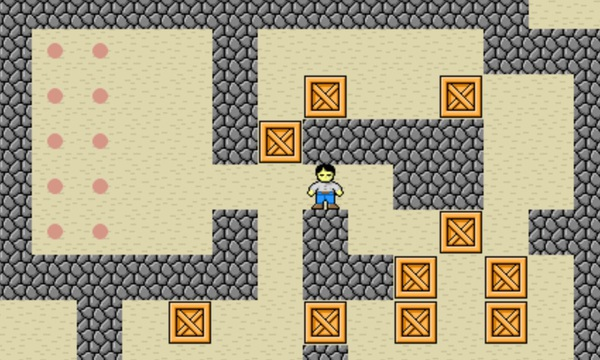
\includegraphics[width=0.75\textwidth]{sokoban-1735.jpg}
    \caption{Jeu de Sokoban}
    
\end{figure}

\newpage

\tableofcontents

\newpage

\section*{Introduction}


\addcontentsline{toc}{section}{Introduction}
Le but de ce projet est d'implementer en langage de programmation C le jeu 'SOKOBAN'.
\newline
Seules certaines parties du code seront présentées ici, et nous avons notamment pris soin d'omettre les aspects les plus mondains ou encombrants du code, comme l’allocation et la libération de la mémoire, la déclaration de certaines variables, certaines fonctions
auxiliaires, la validation des inputs, quelques affichages console, et les demandes d’input via console. L’ensemble du programme offre plus de rigueur, et nous nous sommes efforcés de fournir du code propre et lisible quand nous en étions capables.

\subsection{Règles du jeu}
Les règles du jeu que l’on souhaite implémenter sont les suivantes :
Nous disposons d’un plateau de jeu constitué de murs et de cases libres. Nous pouvons déplacer
un personnage dans les 4 directions (haut, bas, gauche et droite) pourvu que la case visée ne
soit pas un mur.
Sur le plateau sont disposés des caisses et des points d’intérêts sur des cases particulières. Le but étant de couvrir par des caisses tous les points d´esign´es. Pour ce faire le personnage peut
déplacer les caisses en les poussant. Cependant, pour pouvoir d´eplacer une caisse, il faut qu’il y
ait une case libre de part et d’autre de la caisse. Si par exemple le personnage est à droite de la caisse et qu’une case est libre à gauche de la caisse, le personnage pourra déplacer la caisse vers la gauche. Ainsi une fois que la caisse est contre un mur, il est souvent difficile de la décoller du mur.

\subsection{Plateau de jeu}

Pour représenter le plateau de jeu, nous avons décidé d'utiliser un tableau à deux dimensions de taille $20\times20$. Il s'agit d'un tableau d'entiers :
\begin{itemize}
    \item \textbf{-1} représente un \textbf{mur}
    \item \textbf{0} représente un \textbf{casse vide}
    \item \textbf{1} représente le \textbf{personnage}
    \item \textbf{2} représente une \textbf{caisse}
    \item \textbf{3} représente un \textbf{objectif}
    \item \textbf{4} représente le \textbf{personnage sur un objectif}
    \item \textbf{5} représente une \textbf{caisse sur un objectif}\\
   
\end{itemize}
On a choisi cette méthode car nous pensons qu'elle est plus facile à traiter et moins coûteuse en temps.

\subsection{Fonctionnalités}

A travers notre jeu, nous avons mis en place plusieurs fonctionnalités :\\
\begin{itemize}
    \item le jeu en lui-même, c'est-à-dire la possibilité de bouger le personnage et de pousser les caisses sur des objectifs
    \item des niveaux avec un ordre de difficulté et la possibilité de naviguer entre eux
    \item un système de détection de fin de niveau pour savoir quand le joueur a gagné ou est bloqué
    \item un chronomètre, commençant lorsque la partie débute et se mettant à jour à chaque input
    \item un système de score basé sur le nombre d'input du joueur et du temps écoulé
    \item un système de sauvegarde permettant au joueur de reprendre sa partie où il l'a laissée\\
   
\end{itemize}
\section{Structure du code}
Nous avons structuré le code de jeu dans trois fichiers principaux:
\begin{itemize}
    \item 1. Le fichier \textbf{"inc"} qui contient les fonctions utilisées pour le jeu.
    \item 2. Le fichier \textbf{"map"} qui contient tous les plateux possibles de jeu pour chaque niveau.
    \item 3. Le fichier \textbf{"src"} qu'on a developpé tous les fonctions du jeu. 
\end{itemize}
\section{Implémentation des fonctionnalités}
\subsection{Affichage}

Ici, nous allons répertorier toutes les fonctions liés à l'affichage du plateau lors du jeu. A noter que \textbf{\#} représente un mur, \textbf{P} le personnage, \textbf{c} une caisse, \textbf{ç} une caisse sur un objectif, \textbf{I} un objectif et \textbf{ } une casse vide.\\\\

\textbf{affichage(...):}
\begin{itemize}
\item Est une fonction qui affiche le plateau du jeu.
\end{itemize}

Signature de fonction :
\begin{lstlisting}
void affichage(int **plateau, int taille);
\end{lstlisting}

\textbf{affiche-score(...):}
\begin{itemize}
\item Est une fonction qui affiche le score.
\end{itemize}
Signature de fonction :
\begin{lstlisting}
void affiche_score(int best_score, int score);
\end{lstlisting}
\newpage
\subsection{Déplacement}
Ici, nous allons vous expliquer toutes les fonctions en charge du déplacement du personnage à travers le plateau. Le joueur peut le faire grâce aux touches \textbf{z,q,s,d}.\\\\
\textbf{deplacement-possible(...):}
\begin{itemize}
\item Fonction renvoyant si le deplacement d'une entite est possible dans une telle direction.
\item Si entite = 1 alors on s'interesse au personnage si = a 2 il s'agit d'une caisse.
\item x,y sont les coordonnees de l'entite dans le tableau.
\item La fonction renvoie 1 si deplacement possible, 0 sinon.
\end{itemize}
Signature de fonction :
\begin{lstlisting}
int deplacement_possible(int **plateau, int taille, int x, int y, char direc, int entite);
\end{lstlisting}
\textbf{maj-carte(...):}
\begin{itemize}
\item Cette fonction met à jour les valeurs des cases du tableau selon les dépalcements effectués
\item Elle prend en argument, le plateau, les coordonnées du personne.
\item depla-x indique si le perso bouge de façon verticale(-1 s'il monte, +1 s'il descend)au.
\item depla-y indique si le perso bouge de façon horizontale(-1 s'il va à gauche, +1 s'il va à droite.
\end{itemize}
Signature de fonction :
\begin{lstlisting}
void maj_carte(int ** plateau, int *x, int *y, int depla_x, int depla_y);
\end{lstlisting}
\textbf{deplacememt(...):}
\begin{itemize}
\item Cette fonction s'occupe de gérer le déplacement du personnage dans le tableau.
\item En plus elle sert aussi à compter le nombre de tours utiles pour le calcul du score.
\end{itemize}
Signature de fonction :
\begin{lstlisting}
void deplacememt(int direc, int ** plateau, int taille, int *x, int *y, int *nb_tours);
\end{lstlisting}
\textbf{detect-fin(...):}
\begin{itemize}
\item Cette fonction sert à détecter une fin de jeu.
\item Elle renvoie 1 si tous les objectifs ont été complété.
\item Elle renvoie 0 si la partie est toujours en cours.
\item Elle renvoie -1 si le joueur est bloqué.
\end{itemize}
Signature de fonction :
\begin{lstlisting}
int detect_fin(int **plateau, int taille);
\end{lstlisting}


\newpage

\subsection{Sauvegarde/Chargement}
Ici, nous détaillerons comment fonctionne le système de sauvegarde et de chargement de la sauvegarde et d'un niveau.\\
Les niveaux sont stockés dans le répertoire \textbf{./maps} et sont des fichiers du nom \textbf{"map$x$.txt"} avec $x$ étant le numéro du niveau. Chaque fichier contient une suite de 400 entiers représentant la map de jeu.\\
Le fichier \textbf{save.txt} est aussi dans le même répertoire et contient la dernière sauvegarde faite par le joueur (le fichier n'existe pas si le joueur n'a jamais sauvegardé). Le fichier est de la même forme que ceux contenant les maps, hormis qu'au début de celui-ci sont aussi stockés le numéro du niveau, le temps écoulé lors de la partie et le score de la partie.\\
\newline
\textbf{save(...):}
\begin{itemize}
\item Cette fonction permet de sauvegarder la progression dans le fichier \textbf{save.txt}.
\item Elle note le temps auquel la sauvegarde a été faite, le nombre de tours écoulés durant la partie, et le niveau.
\end{itemize}
Signature de fonction :
\begin{lstlisting}
void save(int** plateau, int niveau, int time, int nb_tours);
\end{lstlisting}
\textbf{charger(...):}
\begin{itemize}
\item Cette fonction permet de charger un niveau.
\end{itemize}
Signature de fonction :
\begin{lstlisting}
void charger(int *num_niveau, int **plateau, int *x, int *y, int charge_save, int *time, int *nb_tours);
\end{lstlisting}
\textbf{if\_file\_exist(...):}
\begin{itemize}
\item Cette fonction permet de contrôler si un fichier existe.
\end{itemize}
Signature de fonction :
\begin{lstlisting}
int if_file_exist(char *fichier);
\end{lstlisting}
\newpage

\subsection{Menu/Niveaux}
Ici, nous allons détailler les fonctions utilisées pour l'affichage du menu et le déplacement entre les niveaux lors de la partie.
\newline
\textbf{menu(...):}
\begin{itemize}
\item Cette fonction affiche le menu et permettant au joueur de choisir ce qu'il veut faire.
\item Les options de joueur sont: 
\begin{itemize}
\item Si le joueur appuye "1", il va commencer une nouvelle partie.
\item Si le joueur appuye "2", il va changer la partie.
\item Si le joueur appuye "3", les régles de jeu seront affichées.
\item Si le joueur appuye "4", il quitte le jeu.
\end{itemize}
\end{itemize}
Signature de fonction :
\begin{lstlisting}
void menu(int ** plateau, int *score_tab);
\end{lstlisting}
\textbf{lance-niveau(...):}
\begin{itemize}
\item Cette focntion permet de lancer le niveau voulu.
\item \textit{charger\_niveau} permet de savoir si on charge le fichier sauvegardé ou non.
\end{itemize}
Signature de fonction :
\begin{lstlisting}
void lance_niveau(int num_niveau, int ** plateau,int charger_niveau, int *score_tab);
\end{lstlisting}
\textbf{fin-niveau(...):}
\begin{itemize}
\item Cette fonction gére la transition entre les niveaux.
\item Si l'utilisateur a terminé un niveau, le programme lui demande s'il veut continuer au niveau suivant ou non.
\item Si l'utilisateur a terminé le jeu le programme lui demande s'il veut revenier au 1er niveau ou retourner au menu.
\item Si l'utilisateur a perdu le niveau, le programme lui demande s'il veut retenter le niveau ou retourner au menu.
\end{itemize}
Signature de fonction :
\begin{lstlisting}
void fin_niveau(int fin,int num_niveau, int **plateau, int *score_tab);
\end{lstlisting}
\textbf{regles():}
\begin{itemize}
\item Cette fonction affiche tous les règles de jeu et les instructions.
\end{itemize}
Signature de fonction :
\begin{lstlisting}
void regles();
\end{lstlisting}
\newpage

\subsection{Chronomètre}
Ici, nous allons expliquer les fonctions permettant le fonctionnnement du chronomètre ainsi que son affichage.
A noter, que le chronomètre n'est pas en temps réel mais qu'il se met à jour à chaque input par l'utilisateur.\\

\textbf{get\_time(...):}
\begin{itemize}
\item Cette fonction renvoie dans une variable \textbf{time\_t}, le moment où elle est appelée.
\item \textbf{time\_t} représente le temps écoulé depuis le $1^{er}$ janvier 1970 à 00:00:00.
\end{itemize}
Signature de fonction :
\begin{lstlisting}
time_t get_time();
\end{lstlisting}

\textbf{affiche\_timer(...):}
\begin{itemize}
\item Cette fonction affiche le chronomètre lors de la partie.
\item Il est de la forme \textbf{heures:minutes:secondes}. Pour chaque, deux chiffres sont affichés.
\item Le paramètre \textit{start} contient le moment auquel la partie a commencé.
\item Quand la fonction est appelée, on fait appel à la fonction \textbf{get\_time}. On fait ensuite la différence avec la valeur contenue dans \textit{start}. On obtient un résultat en secondes.
\item Le paramètre \textit{decalage} contient la valeur obtenue dans le fichier sauvegarde. Comme ça le chronomètre commence aura au commencement la même valeur que lors de la sauvegarde.
\end{itemize}
Signature de fonction :
\begin{lstlisting}
void affiche_timer(time_t start, int *diff_int, int decalage);
\end{lstlisting}
\newpage

\subsection{Score}
Ici, nous détaillerons la fonctionnalité du score et sa mise en place dans le jeu.\\ 
Un fichier \textbf{score.txt} permet au joueur de voir son meilleur score à chaque niveau. Celui-ci est formaté et initialisé à 0 pour chaque score. Lorsque le joueur termine un niveau et qu'il a battu son meilleur score, le fichier est mis à jour.\\
Le calcul du score se fait par la formule suivante :
\begin{equation}
    score = 1000*num\_niveau - (temps\_ecoule*nombre\_tours\_ecoules)
\end{equation}

\textbf{calcule\_score(...):}
\begin{itemize}
\item Cette fonction calcule le score à un instant t de la partie selon la formule vu au-dessus.
\end{itemize}
Signature de fonction :
\begin{lstlisting}
int calcule_score(int nb_tours, int temps, int num_niveau);
\end{lstlisting}

\textbf{get\_best\_score(...):}
\begin{itemize}
\item Cette fonction récupère les scores stockés dans le document \textbf{score.txt} et les range dans le tableau passé en paramètre.
\end{itemize}
Signature de fonction :
\begin{lstlisting}
void get_best_score(int *tab);
\end{lstlisting}

\textbf{maj\_best\_score(...):}
\begin{itemize}
\item Cette fonction permet quant à elle de changer le score du niveau passé en paramètre dans le fichier. \textbf{score.txt}.
\item La valeur est aussi remplacée dans le tableau.
\end{itemize}
Signature de fonction :
\begin{lstlisting}
void maj_best_score(int* score_tab, int best_score, int num_niveau);
\end{lstlisting}

\textbf{fichier\_score(...):}
\begin{itemize}
\item Cette fonction crée le fichier \textbf{score.txt}, utile s'il est supprimé par erreur.
\end{itemize}
Signature de fonction :
\begin{lstlisting}
void fichier_score();
\end{lstlisting}

\newpage


\listoffigures

\end{document}


